
    
    
\documentclass{article}
\usepackage[utf8]{inputenc}
\usepackage{graphicx}
\usepackage[T1]{fontenc}
\usepackage{lmodern}
\usepackage{listings}
\usepackage[numbers]{natbib} %IEEE
\usepackage{color}
\usepackage{hyperref}
\usepackage{soul}
\usepackage{float}
\usepackage{pgfplotstable}
\usepackage[font=itshape]{quoting}
\usepackage{booktabs}
\usepackage{amsmath}
\usepackage{multicol}
%\usepackage[table,xcdraw]{xcolor}
\setcounter{MaxMatrixCols}{11}


\usepackage{minted}
\usepackage[a4paper, total={6.5in, 8in}]{geometry}
\definecolor{dkgreen}{rgb}{0,0.6,0}
\definecolor{gray}{rgb}{0.5,0.5,0.5}
\definecolor{mauve}{rgb}{0.58,0,0.82}
\definecolor{backcolour}{rgb}{0.95,0.95,0.92}
\definecolor{codegreen}{rgb}{0,0.6,0}
% Define a custom style
\lstdefinestyle{myStyle}{
    backgroundcolor=\color{backcolour},   
    commentstyle=\color{codegreen},
    keywordstyle = \bfseries\color{mauve},
    basicstyle=\ttfamily\footnotesize,
    breakatwhitespace=false,         
    breaklines=true,                 
    keepspaces=true,                 
    numbers=left,       
    numbersep=5pt,                  
    showspaces=false,                
    showstringspaces=false,
    showtabs=false,                  
    tabsize=2,
}
\lstset{style=mystyle}

\title{Data Mining \& Machine Learning \\ \large Computer Exercise 6 - Neural Networks \& PyTorch}
\author{Steinarr Hrafn Höskuldsson}
\date{September 2022}
\newcommand{\mycomment}[1]{}

\begin{document}
\maketitle

\mycomment{
\begin{figure}[h]
    \centering
    \includegraphics[width=0.75\textwidth]{LAB3/Basic1.png}
    \caption{"Switch test" Breadboard set up}
    \label{fig:Switch_test}
\end{figure}

\lstinputlisting[caption=Defining 'ColorMatch' state, label={lst:colormatch}, language=Python, firstline=44, lastline=52]{LAB3/Basic.py}
}
\section*{Section 1}
I moved the training to my laptops GPU and added significantly more neurons to both the convolutional layers and the first linear layer. The total accuracy of the network increased from 52\% as it was in the training example to 65\%. The misclassification rates for each for each category was plotted and can be seen in Figure \ref{fig:misclass}
\begin{figure}[h]
    \centering
    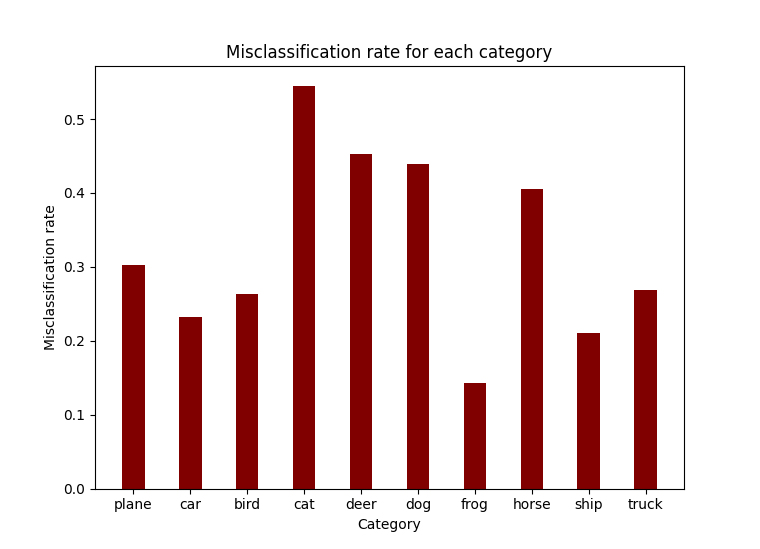
\includegraphics[width=0.75\textwidth]{06_neural_networks/1.png}
    \caption{Misclassification rate of each category}
    \label{fig:misclass
    }
\end{figure}
\newpage
The Confusion matrix was calculated.
\begin{center}
CM = 
\begin{bmatrix}
     &plane & car & bird & cat & deer & dog & frog & horse & ship & truck\\
    plane & 765 & 23 & 16 & 29 & 20 & 3 & 4 & 21 & 74 & 45\\
car & 16 & 839 & 3 & 13 & 4 & 4 & 3 & 4 & 22 & 92\\
bird & 113 & 20 & 350 & 98 & 147 & 110 & 43 & 81 & 19 & 19\\
cat & 33 & 13 & 25 & 499 & 75 & 205 & 21 & 87 & 19 & 23\\
deer & 15 & 4 & 34 & 70 & 595 & 37 & 16 & 206 & 19 & 4\\
dog & 13 & 6 & 17 & 169 & 49 & 607 & 5 & 116 & 5 & 13\\
frog & 7 & 14 & 21 & 156 & 148 & 37 & 578 & 18 & 15 & 6\\
horse & 17 & 0 & 6 & 26 & 41 & 63 & 2 & 817 & 3 & 25\\
ship & 80 & 43 & 2 & 22 & 5 & 10 & 0 & 3 & 787 & 48\\
truck & 38 & 131 & 1 & 14 & 4 & 6 & 2 & 22 & 34 & 748
    \end{bmatrix}
\end{center}
In the confusion matrix one can spot that the most common misclassifcations were mix ups of dog/cat, bird/plane, car/truck, horse/deer/frog which suggests the network might be relying on the background to some extent to classify. Perhaps if the training data also included images with the background extracted the networks could performance could be improved.

The training of the network in PyTorch relied heavily on the AutoGrad which is PyTorch's automatic differentation engine. It keeps track of operations performed on the dataflow and knows the derivative of those events. When needed, it can apply the chain rule to compute the partial derivative in question.

\section*{Section 2}
RNN stand for Recursive Neural Network. The recursiveness comes from the fact that the part of the input into the network is the output from the last run. This allows the network to remember what was going on. RNN's are very useful in situations where something is happening over time and the network has to remember what has already happened. A good example of such a situation is working with text. A very important part of having a conversation or completing a sentence is remembering what has previously been said. Other use cases for RNNs are for example video analysis, speech recognition and sequence prediction.

\\
A RNN network was trained based on the example from Pytorch's tutorial. In my opinion the RNN model in Pytorch's example did not perform very well. Although the made up names are usually phonetically viable, they usually did not sound like real names.

\newpage

\section*{Independent Section}
All icelandic given names were downloaded from \hyperlink{https://opingogn.is/dataset/mannanafnaskra/resource/27dc8c43-247e-4797-a603-87853637e038}{opinskra.is}. A short python program was written to parse the valid ones into a .txt file. The Name generation example was then run again and the output generated for Icelandic names was as follows:

\begin{itemize}
    \item Sari
    \item Tring
    \item Ering
    \item Irin
    \item Nari
    \item Arrin
    \item Rongani
    \item Rimar
\end{itemize}

And to a native Icelandic speaker such as myself, none of those sound like an actual name except for the last one, Rimar, which fooled me, I had to look up that it is indeed not a name.

\newpage
\section*{Appendix}
\appendix
\section{Code}

\lstinputlisting[ label={lst:colormatch}, language=Python, ]{05_backprop/Steinarr5.py}


\end{document}

